% Options for packages loaded elsewhere
\PassOptionsToPackage{unicode}{hyperref}
\PassOptionsToPackage{hyphens}{url}
\PassOptionsToPackage{dvipsnames,svgnames*,x11names*}{xcolor}
%
\documentclass[
]{book}
\usepackage{lmodern}
\usepackage{amssymb,amsmath}
\usepackage{ifxetex,ifluatex}
\ifnum 0\ifxetex 1\fi\ifluatex 1\fi=0 % if pdftex
  \usepackage[T1]{fontenc}
  \usepackage[utf8]{inputenc}
  \usepackage{textcomp} % provide euro and other symbols
\else % if luatex or xetex
  \usepackage{unicode-math}
  \defaultfontfeatures{Scale=MatchLowercase}
  \defaultfontfeatures[\rmfamily]{Ligatures=TeX,Scale=1}
\fi
% Use upquote if available, for straight quotes in verbatim environments
\IfFileExists{upquote.sty}{\usepackage{upquote}}{}
\IfFileExists{microtype.sty}{% use microtype if available
  \usepackage[]{microtype}
  \UseMicrotypeSet[protrusion]{basicmath} % disable protrusion for tt fonts
}{}
\makeatletter
\@ifundefined{KOMAClassName}{% if non-KOMA class
  \IfFileExists{parskip.sty}{%
    \usepackage{parskip}
  }{% else
    \setlength{\parindent}{0pt}
    \setlength{\parskip}{6pt plus 2pt minus 1pt}}
}{% if KOMA class
  \KOMAoptions{parskip=half}}
\makeatother
\usepackage{xcolor}
\IfFileExists{xurl.sty}{\usepackage{xurl}}{} % add URL line breaks if available
\IfFileExists{bookmark.sty}{\usepackage{bookmark}}{\usepackage{hyperref}}
\hypersetup{
  pdftitle={Metoda reprezentacyjna},
  pdfauthor={Łukasz Wawrowski},
  colorlinks=true,
  linkcolor=Maroon,
  filecolor=Maroon,
  citecolor=Blue,
  urlcolor=Blue,
  pdfcreator={LaTeX via pandoc}}
\urlstyle{same} % disable monospaced font for URLs
\usepackage{longtable,booktabs}
% Correct order of tables after \paragraph or \subparagraph
\usepackage{etoolbox}
\makeatletter
\patchcmd\longtable{\par}{\if@noskipsec\mbox{}\fi\par}{}{}
\makeatother
% Allow footnotes in longtable head/foot
\IfFileExists{footnotehyper.sty}{\usepackage{footnotehyper}}{\usepackage{footnote}}
\makesavenoteenv{longtable}
\usepackage{graphicx}
\makeatletter
\def\maxwidth{\ifdim\Gin@nat@width>\linewidth\linewidth\else\Gin@nat@width\fi}
\def\maxheight{\ifdim\Gin@nat@height>\textheight\textheight\else\Gin@nat@height\fi}
\makeatother
% Scale images if necessary, so that they will not overflow the page
% margins by default, and it is still possible to overwrite the defaults
% using explicit options in \includegraphics[width, height, ...]{}
\setkeys{Gin}{width=\maxwidth,height=\maxheight,keepaspectratio}
% Set default figure placement to htbp
\makeatletter
\def\fps@figure{htbp}
\makeatother
\setlength{\emergencystretch}{3em} % prevent overfull lines
\providecommand{\tightlist}{%
  \setlength{\itemsep}{0pt}\setlength{\parskip}{0pt}}
\setcounter{secnumdepth}{5}
\usepackage{booktabs}
\usepackage{amsthm}
\makeatletter
\def\thm@space@setup{%
  \thm@preskip=8pt plus 2pt minus 4pt
  \thm@postskip=\thm@preskip
}
\makeatother
\usepackage[]{natbib}
\bibliographystyle{apalike}

\title{Metoda reprezentacyjna}
\author{Łukasz Wawrowski}
\date{}

\begin{document}
\maketitle

{
\hypersetup{linkcolor=}
\setcounter{tocdepth}{1}
\tableofcontents
}
\listoftables
\listoffigures
\hypertarget{literatura}{%
\chapter*{Literatura}\label{literatura}}
\addcontentsline{toc}{chapter}{Literatura}

\begin{itemize}
\tightlist
\item
  Heeringa, S. G., West, B. T., \& Berglund, P. A. (2017). Applied survey data analysis. CRC press.
\item
  Lumley, T. (2011). Complex surveys: a guide to analysis using R. John Wiley \& Sons.
\item
  Falissard, B. (2011). Analysis of questionnaire data with R. CRC Press.
\item
  De Leeuw, E. D., Hox, J. J., \& Dillman, D. A. (2008). International handbook of survey methodology. Taylor \& Francis Group.
\end{itemize}

\hypertarget{wprowadzenie-do-metody-reprezentacyjnej}{%
\chapter{Wprowadzenie do metody reprezentacyjnej}\label{wprowadzenie-do-metody-reprezentacyjnej}}

\href{https://docs.google.com/presentation/d/1U-vMmSwtyOHihqkImD5gSmuTuksHvnUhGHXcMESNOS8/edit?usp=sharing}{Prezentacja}

\hypertarget{metoda-reprezentacyjna}{%
\section{Metoda reprezentacyjna}\label{metoda-reprezentacyjna}}

Badania statystyczne stanowią podstawę funkcjonowania państwa oraz społeczeństwa - dzięki nim znany jest poziom inflacji czy bezrobocia. W praktyce dominują badania oparte na próbie, ponieważ badanie wszystkich jednostek często jest utrudnione oraz nieopłacalne. Dzięki zastosowaniu odpowiednich metod statystycznych wyniki zebrane na podstawie próby można z powodzeniem uogólniać na całą populację. Oczywiście znając wielkość błędu jaki się wówczas popełnia.

Metoda reprezentacyjna ma na celu określenie zasad dotyczących projektowania, zbierania, przetwarzania oraz analizy danych, które wpływają na koszt i jakość badania. Innymi słowy metoda reprezentacyjna zajmuje się metodologią badań statystycznych.

W Polsce prym w prowadzeniu badań wiedzie Główny Urząd Statystyczny, który w \href{https://bip.stat.gov.pl/dzialalnosc-statystyki-publicznej/program-badan-statystycznych/pbssp-2020/}{Programie Badań Statystycznych Statystyki Publicznej} publikuje listę prowadzonych badań. Oprócz tego na rynku działa wiele firm, które zajmują się badaniami statystycznymi. Wśród najpopularniejszych można wskazać \href{https://www.cbos.pl/PL/home/home.php}{CBOS}, Kantar Millward Brown i wiele innych. Najgłośniej o tych podmiotach mówi się przy okazji wyborów, kiedy na tapetę brane są \href{https://sprawdzamysondaze.pl/}{sondaże}. Z dobrodziejstw badań statystycznych korzystają także prywatne przedsiębiorstwa produkcyjne, które z wykorzystaniem tych metod prowadzą badania jakościowe.

Projektując badanie statystyczne musimy zdefiniować następujące charakterystyki badania:

\begin{enumerate}
\def\labelenumi{\arabic{enumi}.}
\tightlist
\item
  Cel badania
\item
  \textbf{Populacja generalna} którą badanie ma opisywać
\item
  Źródła z których może zostać wylosowana próba - \textbf{operat losowania}
\item
  Sposób w jaki próba zostanie wylosowana - \textbf{schemat losowania}
\item
  Sposób zbierania danych (\href{https://beedifferent.pl/blog/techniki-organizacji-badan-komunikacji-wewnetrznej-cati-cawi-capi-i-papi}{CATI, CAWI, CAPI I PAPI})
\end{enumerate}

Badanie, które przeprowadzimy zgodnie z powyższą listą cechuje się tym, że jest oparte na \textbf{próbie losowej}. Oznacza to, że w sporym uproszczeniu, wyniki badania przeprowadzonego na próbie losowej można uogólniać na populację generalną.

Wśród zalet tego podejścia można wskazać przede wszystkim znajomość wielkości błędu jaki popełniamy przy tym uogólnieniu. Ponadto można wskazać proste zależności pomiędzy liczebnością próby, błędem badania oraz kosztami. Większa liczebność próby implikuje mniejszy błąd badania, natomiast wiąże się ze zwiększeniem kosztów badania. Celem autora badania powinno być znalezienie kompromisu pomiędzy budżetem dostępnym na przeprowadzenie badania a błędem badania.

Do przeprowadzania takiego badania wymagana jest jednak wiedza dziedzinowa oraz dostęp do operatu losowania (czasami jest to poważny problem).

Wcielimy się na chwilę w rolę studentów koła naukowego, które chce przeprowadzić badanie studentów Uniwersytetu Ekonomicznego w Poznaniu na temat wrażeń z ostatniej sesji. Wiadomo, że było super, ale wartoby mieć jakieś liczby, które to potwierdzą.

\begin{enumerate}
\def\labelenumi{\arabic{enumi}.}
\tightlist
\item
  Cel badania: poznanie opinii studentów na wybrany temat.
\item
  Populacja generalna: wszyscy studenci UEP (8415 osób w roku 2018/2019)
\end{enumerate}

Zakładając, że w kole naukowym mamy 10 osób to dotarcie do wszystkich studentów i skłonienie ich do wypełnienia ankiety byłoby problematyczne. Zatem decydujemy się na przeprowadzenia badania na próbie.

\begin{enumerate}
\def\labelenumi{\arabic{enumi}.}
\setcounter{enumi}{2}
\tightlist
\item
  Operat losowania: lista wszystkich studentów UEP wraz z danymi kontaktowymi
\end{enumerate}

W przypadku studentów pozyskanie listy z Biura Obsługi Studentów wraz z dodatkowymi informacji nie powinno być problemem.

\begin{enumerate}
\def\labelenumi{\arabic{enumi}.}
\setcounter{enumi}{3}
\tightlist
\item
  Schemat losowania: wylosowanie z operatu np. 5\% próby z uwzględnieniem płci i kierunku studiów
\end{enumerate}

Najważniejszy moment czyli wybranie osób, które wypełnią naszą ankietę. 5\% z 8415 to około 420 studentów, więc każdy członek koła przeprowadzi wywiad z około 40 studentami - jest to do zrobienia. Powinien być to dobór losowy, ale uwzględniający strukturę np. płci i kierunku studiów. Zależy nam na tym, żeby próba wylosowana do badania była miniaturą populacji.

\begin{enumerate}
\def\labelenumi{\arabic{enumi}.}
\setcounter{enumi}{4}
\tightlist
\item
  Zebranie danych: ankieta w Google Forms
\end{enumerate}

Wysłanie ankiety poprzez e-mail może spowodować, że wiele osób w ogóle nie kliknie w załączony link. Dużo efektywniejszą formą zbierania danych będzie CAPI - wywiad osobisty z wykorzystaniem formularza internetowego.

\hypertarget{rys-historyczny}{%
\section{Rys historyczny}\label{rys-historyczny}}

\textbf{Świat}

\begin{enumerate}
\def\labelenumi{\arabic{enumi}.}
\tightlist
\item
  Booth, C., (1889-1903), \href{https://booth.lse.ac.uk/}{Life and Labour of the People of London}
\end{enumerate}

Zebranie danych o ubóstwie dla każdego domu w Londynie.

\begin{enumerate}
\def\labelenumi{\arabic{enumi}.}
\setcounter{enumi}{1}
\tightlist
\item
  Thurstone, L. i Chave, E., (1929), The Measurement of Attitude, Chicago: University of Chicago.
  Likert, R., (1932), A technique for the measurement of attitudes, Archives of psychology, 140, pp.~5-53.
\end{enumerate}

Wielki kryzys i ograniczone przez to środki przyspieszają rozwój metody reprezentacyjnej. Opracowanie przez Rensisa Likerta pięciostopniowej skali.

\begin{enumerate}
\def\labelenumi{\arabic{enumi}.}
\setcounter{enumi}{2}
\tightlist
\item
  Hansen, M., (1939), Survey of Unemployment.
\end{enumerate}

Pierwsze poważne badanie dotyczące bezrobocia.

\begin{enumerate}
\def\labelenumi{\arabic{enumi}.}
\setcounter{enumi}{3}
\tightlist
\item
  Deming, W., (1950), Some Theory of Sampling, New York: Dover.
  Hansen, M., Hurwitz, W. i Madow, W., (1953), Sample survey methods and theory, Wiley.
\end{enumerate}

Pierwsze podręczniki dotyczące metody reprezentacyjnej.

\textbf{Polska}

Neyman, J., (1933), Zarys teorii i praktyki badania struktury ludności metodą reprezentacyjną

Zasępa, R., (1972), Metoda reprezentacyjna

Bracha, Cz. (1996), Teoretyczne podstawy metody reprezentacyjnej.

\hypertarget{bux142ux119dy}{%
\section{Błędy}\label{bux142ux119dy}}

Na całkowity błąd badania składają się:

\begin{itemize}
\tightlist
\item
  błąd pomiaru i efekt respondenta
\item
  błąd przetwarzania
\item
  błąd pokrycia
\item
  błąd losowania
\item
  błąd braku odpowiedzi
\item
  błąd dopasowania
\end{itemize}

\hypertarget{bux142ux105d-pomiaru-measurement-error}{%
\subsection{Błąd pomiaru (measurement error)}\label{bux142ux105d-pomiaru-measurement-error}}

Jest to różnica pomiędzy tym, co chcemy zmierzyć, a tym co otrzymujemy od respondenta. Np. w pytaniu: \emph{Have you ever, even once, used any form of cocaine?} (National Survey on Drug Use and Health) raczej nie spodziewajamy się szczerych odpowiedzi.

Do tego dochodi response bias (efekt respondenta) czyli wpływ respondenta na otrzymywane wyniki. Przy powtarzalnych badaniach respondenci mogą nauczyć się kwestionariusza i odpowiadać tak, żeby skrócić wywiad.

\hypertarget{bux142ux105d-przetwarzania-processing-error}{%
\subsection{Błąd przetwarzania (processing error)}\label{bux142ux105d-przetwarzania-processing-error}}

Jest to błąd wynikający z analizy odpowiedzi bez szerszego kontekstu oraz błąd kodowania pytań otwartych.

Jeśli podczas analizy kwestionariusza zobaczymy, że ktoś na pytanie \emph{Ile razy dziennie doświadczasz agresji ze strony innych ludzi?} (National Crime Victimization Survey) odpowiedział, że 20 to będziemy mocno zaskoczeni. Nasze zaskoczenie zamieni się w zakłopotanie, kiedy zauważymy, że ta odpowiedź dotyczy respondenta płci męskiej. Na szczęście wykonywany zawód: ochroniarz w klubie nocnym pozwoli na zaakceptowanie takiego stanu rzeczy.

Inną kwestią są pytania otwarte: \emph{Czy w ciągu ostatnich miesięcy słyszałeś o jakichkolwiek zmianach w nastrojach rynkowych?} (Surveys of Consumers). Z racji tego, że występuje trudność w analizie takich pytań często kategoryzuje się taką odpowiedź np. do trzech kategorii: pozytywna, neutralna, negatywna. Problem w tym, że tego przyporządkowania dokonuje pracownik firmy badawczej i często jest to jego subiektywny wybór.

\hypertarget{bux142ux105d-pokrycia-coverage-error}{%
\subsection{Błąd pokrycia (coverage error)}\label{bux142ux105d-pokrycia-coverage-error}}

Polega na objęciu badaniem niekompletnej zbiorowości. Jeżeli za operat losowania przyjęlibyśmy \href{https://pl.wikipedia.org/wiki/Plik:Pierwsza_Polska_Ksi\%C4\%85\%C5\%BCka_Telefoniczna.jpg}{książkę telefoniczną} to badaniem nie obejmiemy osób, które nie posiadają telefonu (populacja nie objęta badaniem). W książce telefonicznej znajdują się także numery do przedsiębiorstw, które będą niekwalifikującymi się jednostkami.

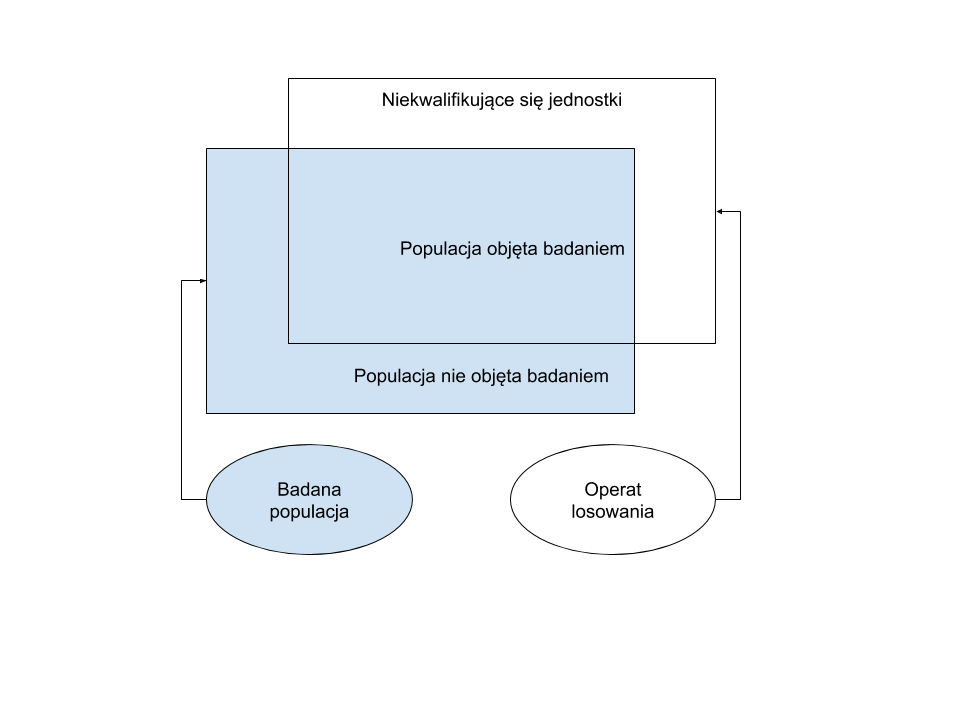
\includegraphics{img/operat.png}

Coverage bias to różnica pomiędzy wynikami dla jednostek objętych i nieobjętych badaniem - w teorii do obliczenia.

\hypertarget{bux142ux105d-losowania-sampling-error}{%
\subsection{Błąd losowania (sampling error)}\label{bux142ux105d-losowania-sampling-error}}

Sampling bias występuje jeżli jednostki w operacie losowania nie mają szans na dostanie się do próby np. ze względu na zbyt małe prawdopodobieństwo wylosowania.

Sampling variance polega na tym, że każdorazowe losowanie próby będzie dawało odmienne wyniki.

\hypertarget{bux142ux105d-braku-odpowiedzi-nonresponse-error}{%
\subsection{Błąd braku odpowiedzi (nonresponse error)}\label{bux142ux105d-braku-odpowiedzi-nonresponse-error}}

Uczniowie nieobecni podczas testu kompetencji z matematyki mogą celowo opuszczać ten dzień w szkole ze względu na świadomość mniejszych umiejętności. Uzyskany przez szkołę wynik będzie z tego względu wyższy niż w przypadku obecności wszystkich uczniów.

\hypertarget{bux142ux105d-dopasowania-adjustement-error}{%
\subsection{Błąd dopasowania (adjustement error)}\label{bux142ux105d-dopasowania-adjustement-error}}

Wykorzystanie danych na temat populacji, wskaźnika kompletności w poprawie jakości próby może spowodować przeszacowanie lub niedoszacowanie wyników dla określonych grup.

  \bibliography{book.bib}

\end{document}
